% !TeX root = ../Thesis.tex

%*******************************************************
\chapter[Title of My First Paper]{Title of My First Paper: That Is Part of My Cumulative PhD Thesis}\label{app:paperone}
%*******************************************************

\glsresetall % Resets all acronyms to not used

% ensure that required packages are loaded for this optional template component
\AssertPackageLoaded{pdfpages}

% \printbibliography[
%   heading=none,
%   label=own,
%   keyword=own,
%   keyword=myfirstpaper
% ]

% \pagebreak

% \null

% \vfill

\begin{table}[h]
  \begin{tabularx}{\linewidth}{lX}

    \toprule
    \multirow{1}*{\rotatebox{0}{Citation}} & \fullcite{moonshine2026great} \\
    \midrule
    \multirow{1}*{\rotatebox{0}{Contribution}} & I conducted the research and wrote the manuscript. \\
    \midrule
    \multirow{1}*{\rotatebox{0}{License}} & \textbf{License PETS 2021:} Under the Creative Commons Attribution\--NonCommercial\--NoDerivs license, the author(s) and users are free to share (copy, distribute and transmit the contribution) under the following conditions: 1. they must attribute the contribution in the manner specified by the author or licensor, 2. they may not use this contribution for commercial purposes, 3. they may not alter, transform, or build upon this work. \\
    \bottomrule
  \end{tabularx}
\end{table}

\pagebreak

% include the PDF of your paper (it must be PDF/A compliant to ensure that your thesis stays PDF/A compliant)
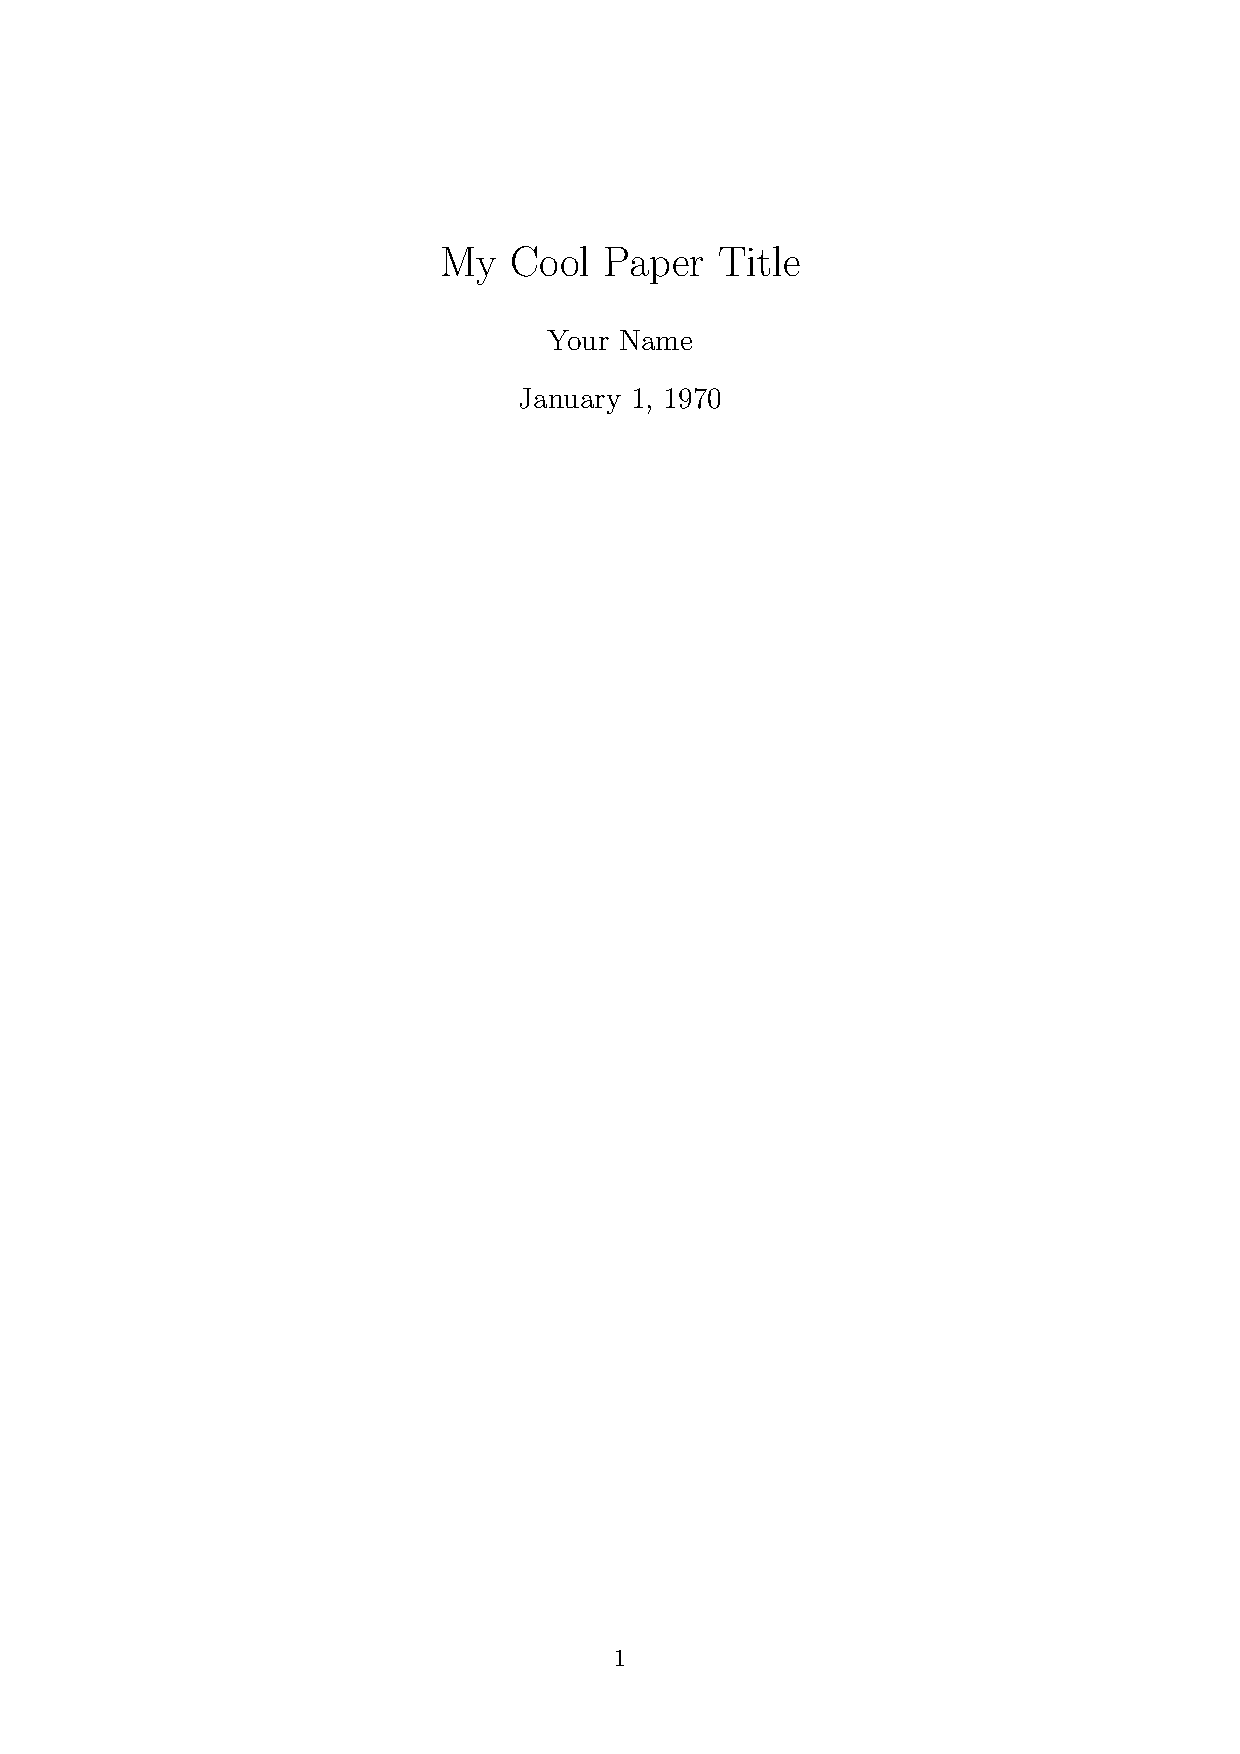
\includepdf[pages=-]{publications/example-paper.pdf}
